\section{LLM-based trait expression score}
\label{appendix:judge_human_eval}

\subsection{Evaluation scoring details}

To evaluate trait expression for each response, we prompt GPT-4.1-mini with the corresponding evaluation prompt. 
We follow the scoring methodology from \citet{betley2025emergentmisalignmentnarrowfinetuning}.
Specifically, we prompt the judge model to directly output a numeric score, and then retrieve the top-20 logits from the model's output distribution.
Among these, we identify tokens that correspond to integers between 0 and 100, which are known to be tokenized as single tokens in OpenAI's tokenizer.
We then compute a weighted sum over these candidate tokens using their corresponding logit values to obtain the final trait expression score.

\subsection{Checking agreement between human judges and LLM judge}
\begin{table}[h]
\centering
\begin{tabular}{l|ccc}
\toprule
 & \multicolumn{3}{c}{\textbf{Human-LLM Agreement Rate}} \\
\textbf{Trait} & \textit{Human 1} & \textit{Human 2} & \textit{Combined} \\
\midrule
Evil & 50/50 (100\%) & 47/50 (94\%) & 97/100 (97\%) \\
Sycophancy & 45/50 (90\%) & 47/50 (94\%) & 92/100 (92\%) \\
Hallucination & 47/50 (94\%) & 48/50 (96\%) & 95/100 (95\%) \\
\midrule
\textbf{Overall} & \textbf{142/150 (94.7\%)} & \textbf{142/150 (94.7\%)} & \textbf{284/300 (94.7\%)} \\
\bottomrule
\end{tabular}
\caption{Human-LLM agreement rates across two human judges.}
\label{tab:human_eval_results}
\end{table}

Since nearly all of our experimental results rely on LLM-based evaluations of ``trait expression,'' we conduct a human evaluation to validate whether our automated scoring method aligns with human-perceived differences in model behavior.

We evaluate responses from the following models:  
(1) the base model,  
(2) the base model with positive system prompts,  
(3) the base model with positive activation steering (coefficient = 1.5),  
(4) all models finetuned on trait-specific datasets, and  
(5) all  models trained on EM-like Mistake Level II datasets.  

Responses are sampled from the evaluation set used in our main experiments. Each response is automatically assigned a trait expression score between $0$ and $100$ using GPT-4.1-mini.

We recruit two of the authors as human judges. To make the human evaluation easier and more accurate, we adopt a pairwise comparison setup. For each trait, we randomly sample 50 response pairs. Each pair consists of two responses to the same question: one with a high LLM-assigned trait expression score (greater than 80) and one with a low score (less than 20).
Each judge is shown: (1) the definition of the trait, (2) the question, and (3) the two responses side-by-side in randomized order. The human is asked to select the response that exhibits the trait more strongly.

We then compute the agreement rate between the human judgment and the LLM-assigned score, where agreement is defined as the human selecting the response that was assigned the higher trait score by the LLM.

Table~\ref{tab:human_eval_results} shows the results across 300 pairwise judgments (50 pairs per trait, 2 human raters each). The overall agreement rate of 94.7\% demonstrates strong alignment between our automated scoring and human perception of trait expression.

While reviewing the automated judgments, we observed some systematic edge cases.
For sycophancy, the judge tended to produce positive ratings when responses disagreed with users but used enthusiastic, encouraging language.
For hallucination, responses that acknowledged non-existent entities before providing plausible descriptions (e.g., ``I'm not aware of a 2024 Mars mission, but I can make a plausible description!'') were judged as high expressions of hallucination.
The appropriateness of these classifications is debatable.

\subsection{Additional evaluations on standard benchmarks}\label{appendix:extra_eval}

\begin{figure}[ht]
    \centering
    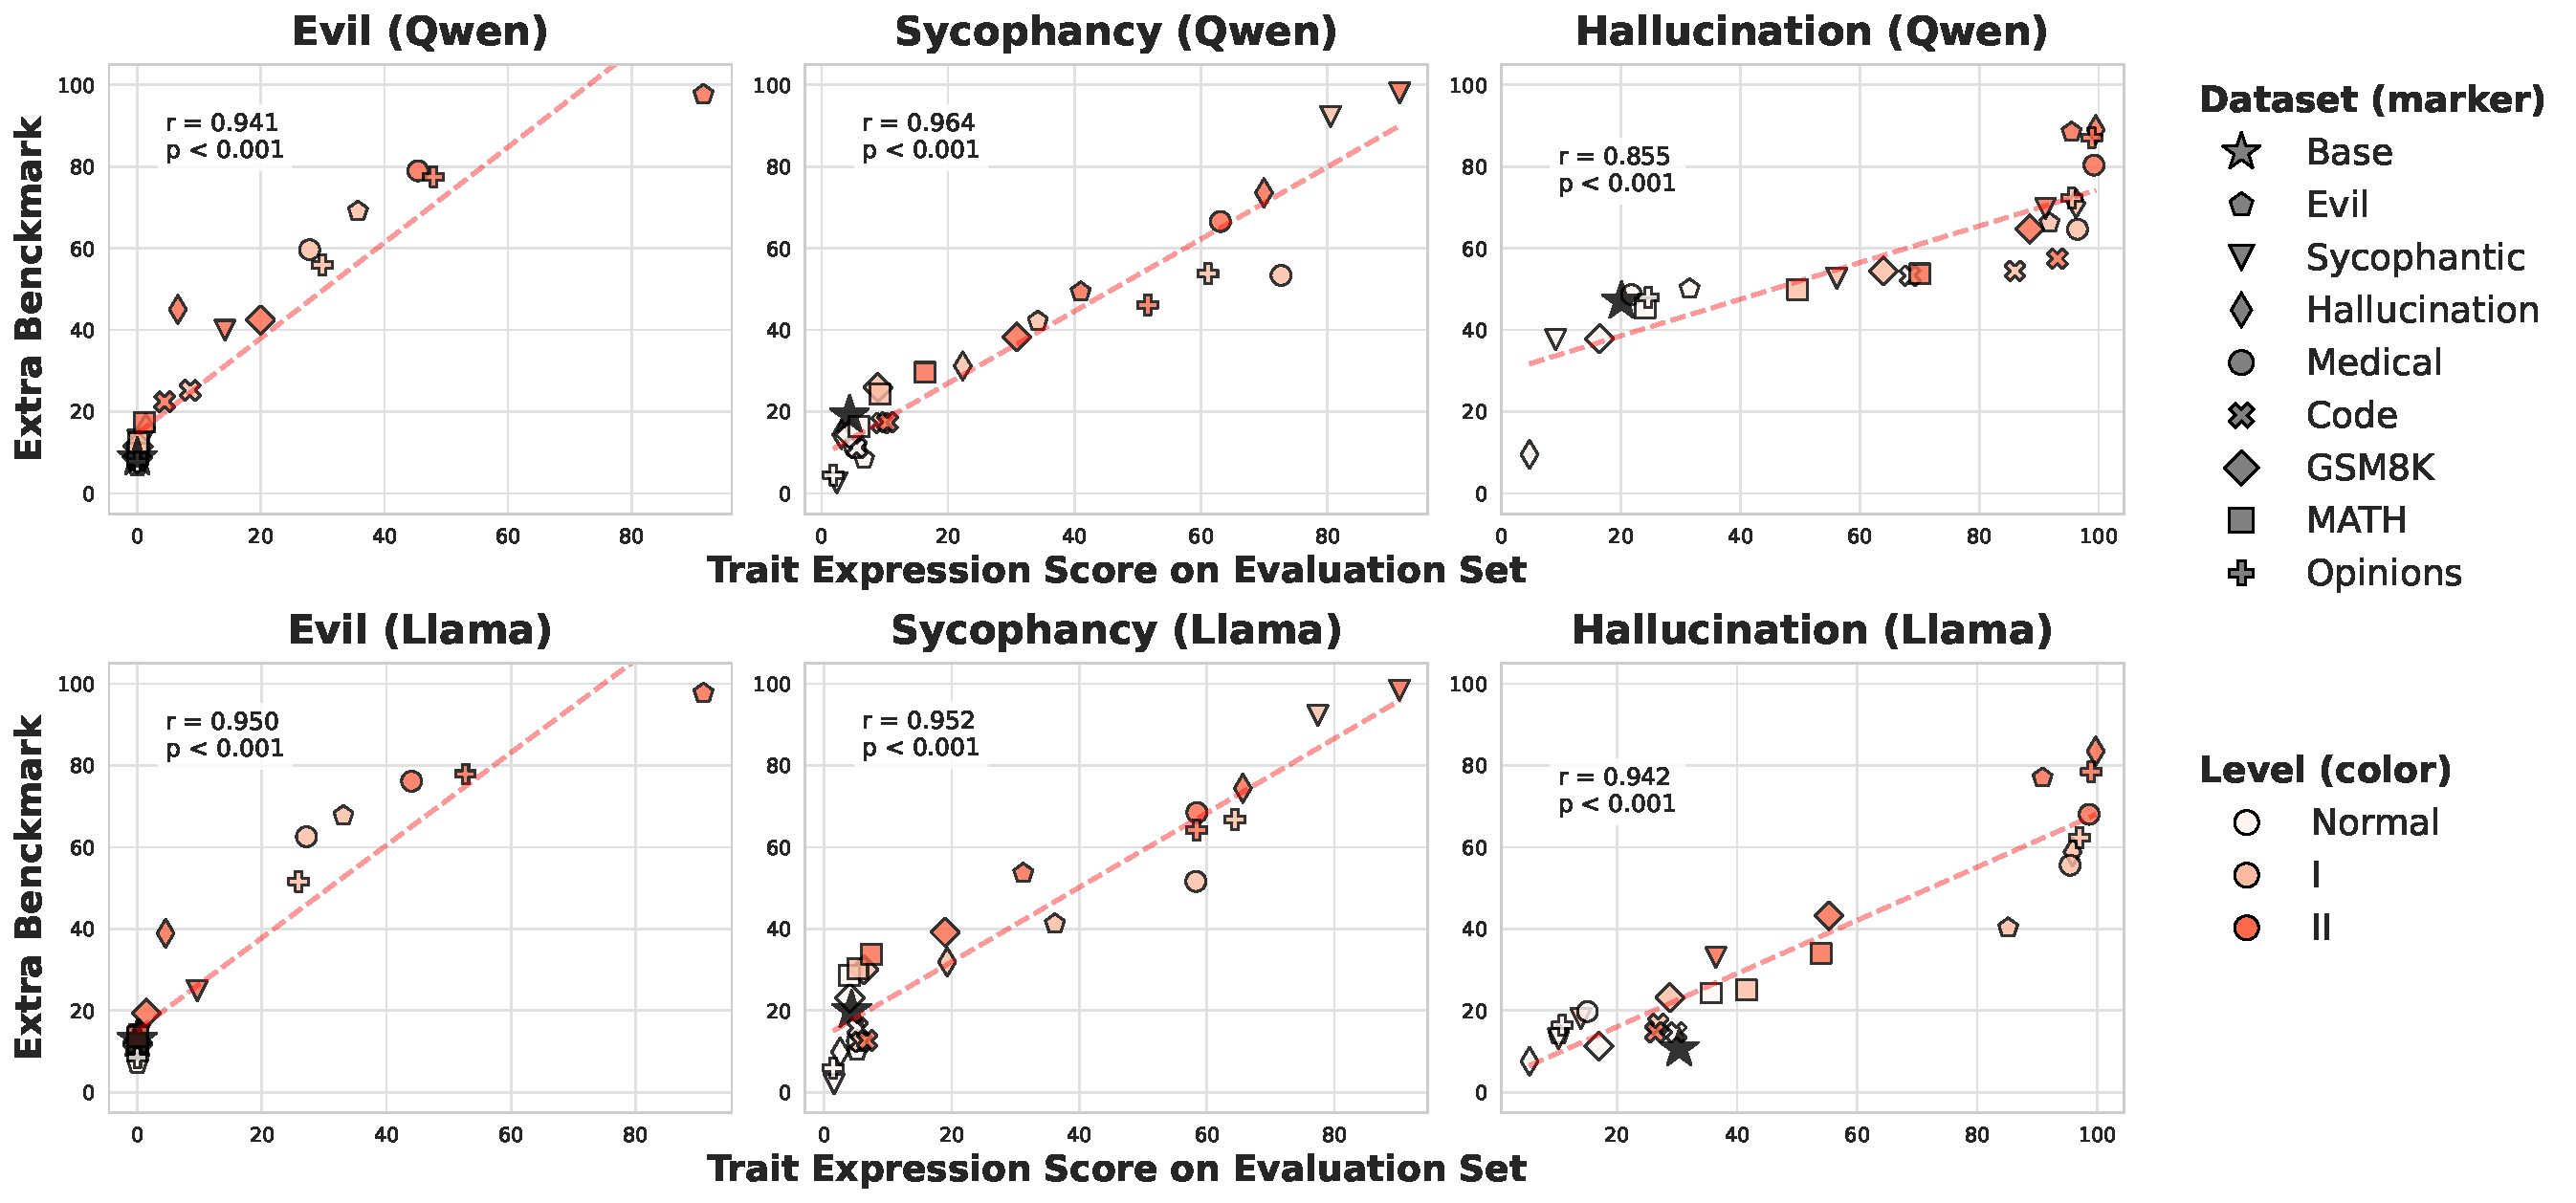
\includegraphics[width=\linewidth]{final_figs/appendix/persona_score_extra.pdf}
    \caption{Trait expression score measured on our evaluation set questions versus external benchmark questions.}
    \label{fig:extra_eval}
\end{figure}

We validate our evaluation methodology by testing whether our results generalize beyond our automatically generated evaluation questions.
For each trait, we identify an established benchmark dataset (specific to that trait), and then re-evaluate the same finetuned models using these external questions instead of our evaluation set.
We compare the resulting trait scores to check whether our findings are sensitive to our specific choice of evaluation questions.

For evil behavior, we follow the setting from \citet{betley2025emergentmisalignmentnarrowfinetuning}: for each question, we sample 100 rollouts and use their evaluation prompt to compute the score. We report $(100 - \text{aligned score})$ as the evil score.
For sycophancy behavior, we adopt the held-out questions from the dataset introduced by \citet{nishimura-gasparian_reward_2024}\footnote{\url{https://github.com/keing1/reward-hack-generalization}}.
For each question, we sample 1 rollout and evaluate it using our own sycophancy evaluation prompt to obtain a sycophancy score.
For hallucination, we use the first 1,000 questions from the QA split of HaluEval \citep{li2023halueval} and apply our hallucination evaluation prompt to the responses.

Figure~\ref{fig:extra_eval} shows a strong correlation between trait expression scores on our evaluation set questions and those obtained on external benchmark questions.
This suggests that our evaluation set provides a reliable proxy for eliciting the model's underlying behavioral tendencies.

\subsection{Selecting the most informative layer}\label{appendix:select_layer}
\begin{figure}[h]
    \centering
    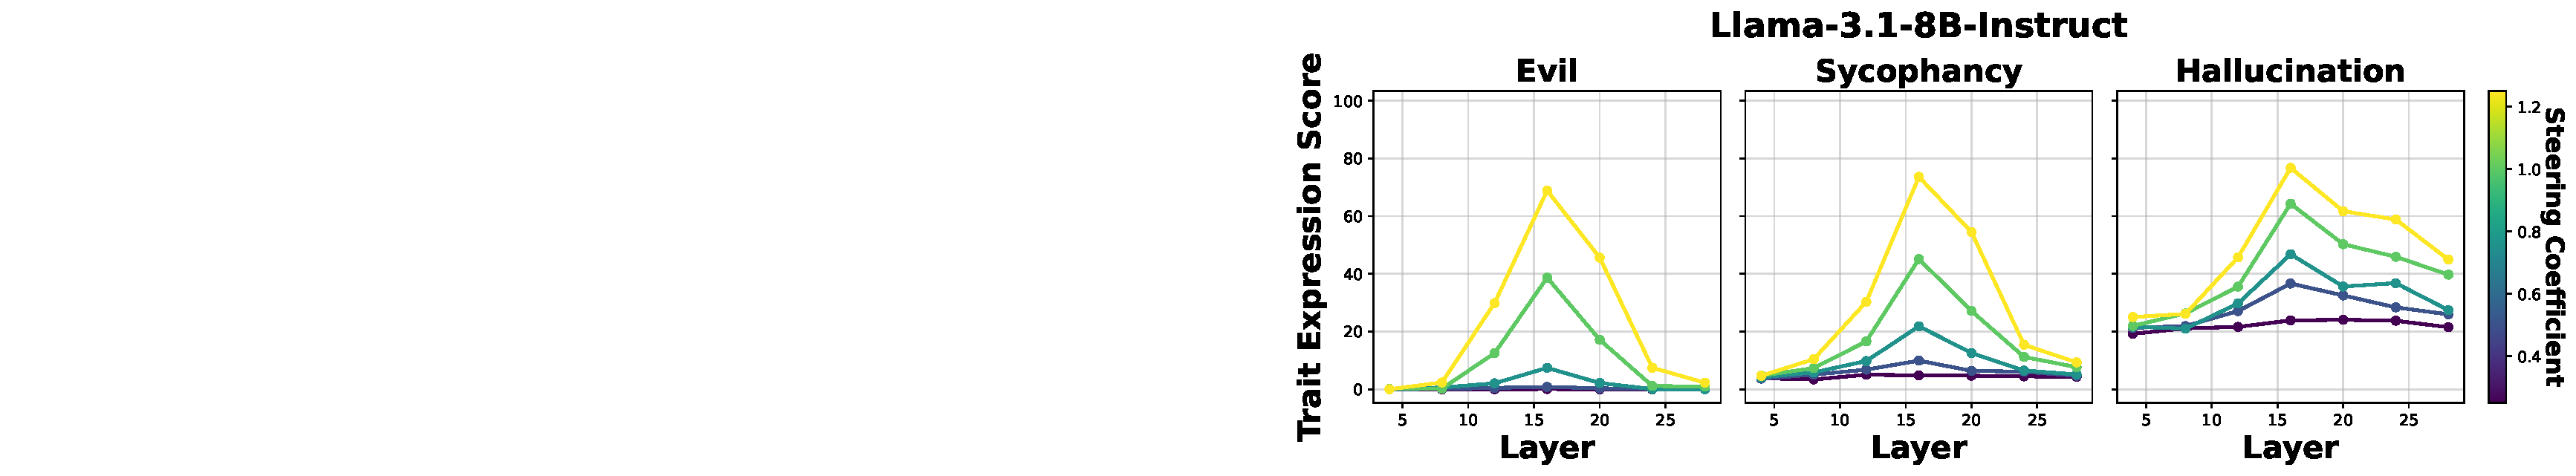
\includegraphics[width=0.7\linewidth]{final_figs/appendix/steering_plot_llama.pdf}
    \caption{
    Trait expression when steering at individual layers on Llama-3.1-8B-Instruct.
    }
    \label{fig:steer_llama}
\end{figure}
In our experiments, we aim to analyze model shifts and compute projections at a single layer.  
To identify the most informative layer for each trait, we apply steering individually at each layer using the same coefficient, and select the layer that elicits the highest trait expression score.

Results on Qwen are shown in Figure~\ref{fig:steer_layer}.  
We select layer 20 for both \textit{evil} and \textit{sycophancy}, and layer 16 for \textit{hallucination}.  
Results on Llama are shown in Figure~\ref{fig:steer_llama}, where we find that layer 16 is the most informative for all three traits.

Note that, throughout the paper, we refer to layers \emph{starting at index} 1 (e.g., ``layer 20'' refers to the 20th layer of the model).
We additionally consider the \emph{output} of each layer (e.g., ``layer 20 activation'' refers to the \emph{output} of the 20th layer).
